\chapter{Implementing the OpenFlow Bundles}
\label{chapter:impl}  
 
\section{Open vSwitch Preparation for OpenFlow 1.4}

The bundles feature that is presented in this paper was introduced by OpenFlow 1.4. In order to add
this new functionality to Open vSwitch, we first had to update the switch to the new protocol version.

The first step was to add protocol definitions to allow the switch to accept the new version. We added
a new header file and updated the build system scripts. These scripts are used to parse the headers
to generate other data structures.

Then we had to update the OpenFlow message handlers. Messages which have the same structure and semantics
in OpenFlow 1.4 as in previous versions were made to use the existing implementation. For the rest of
them, code assertions were used to make sure the switch would not process them.

\section{OpenFlow Bundles}

In order to make our contributions easier to use and to integrate them into Open vSwitch,
we had first to create basic protocol communication handlers for OpenFlow bundles. This
includes encoding and decoding the following message types:
\begin{itemize}
 \item OFPT_BUNDLE_CONTROL
 \item OFPT_BUNDLE_ADD_MESSAGE
\end{itemize}
The first message type is used to open a new bundle, close it, respectively to commit or discard it. The
actual on-the-wire contents of the packet has the structure presented in Figure~\ref{fig:bundle-open-bytes}.

\begin{figure}[h]
\begin{center}
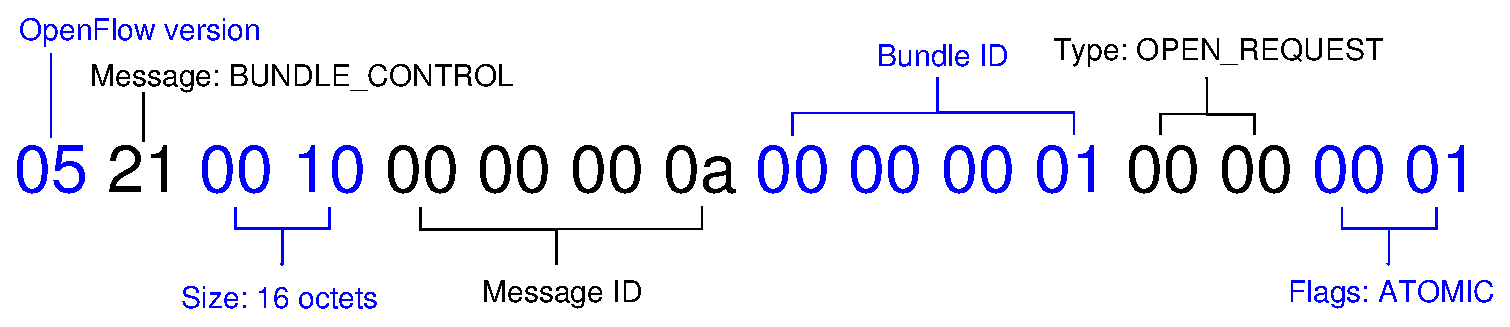
\includegraphics[scale=0.6]{src/img/bundle-open-message-bytes.eps}
\end{center}
\caption{The Structure of an OFPT_BUNDLE_CONTROL Message}
\label{fig:bundle-open-bytes}
\end{figure}

The second message is used after opening a bundle to add messages to it. The same structure applies as for control
messages, but the encpasulated message is added after the main message.

\begin{figure}[h]
\begin{center}
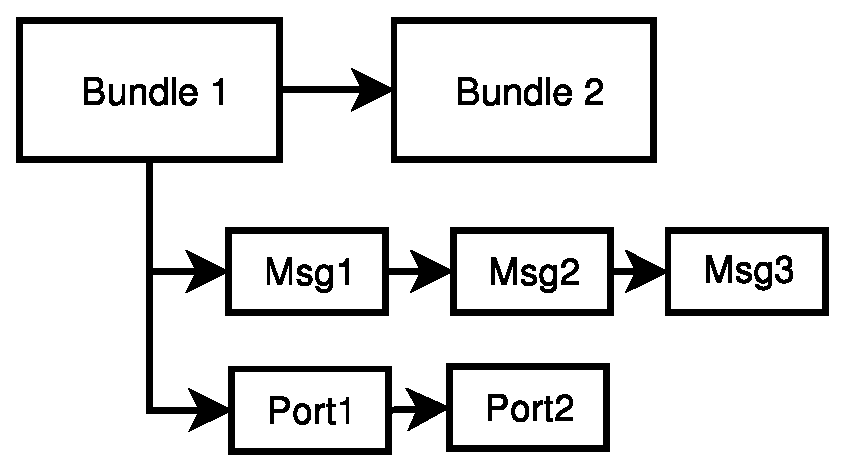
\includegraphics[scale=0.5]{src/img/bundle-content.eps}
\end{center}
\caption{Data Structures Used by a Bundle}
\label{fig:bundles}
\end{figure}

For each OpenFlow connection we may have several bundles open at the same time. Moreover, bundles from different connections
can have the same identifiers. We use a hash table per connection to hold all the active bundles and hashing is done for 
the bundle ID. An example of the data structures that we will be using to implement bundles and the relations between
them are shown in Figure~\ref{fig:bundles}.

A bundle will always be in one the two states shown in Figure~\ref{fig:bundle-state}: \texttt{BS_OPEN} or \texttt{BS_CLOSED}.
Immediately after being created, the bundle is set in the state \texttt{BS_OPEN}. While in this state, messages may be
added to the bundle. When no more messages are required, we can force the bundle to a \texttt{BS_CLOSED} state and not
accept any other message. Another option is to start the commit operation which will automatically close the bundle.
There is also the possibility one of the received messages is invalid. In case of messages that produce errors like that,
the bundle is automatically closed and removed.

\begin{figure}[h]
\begin{center}
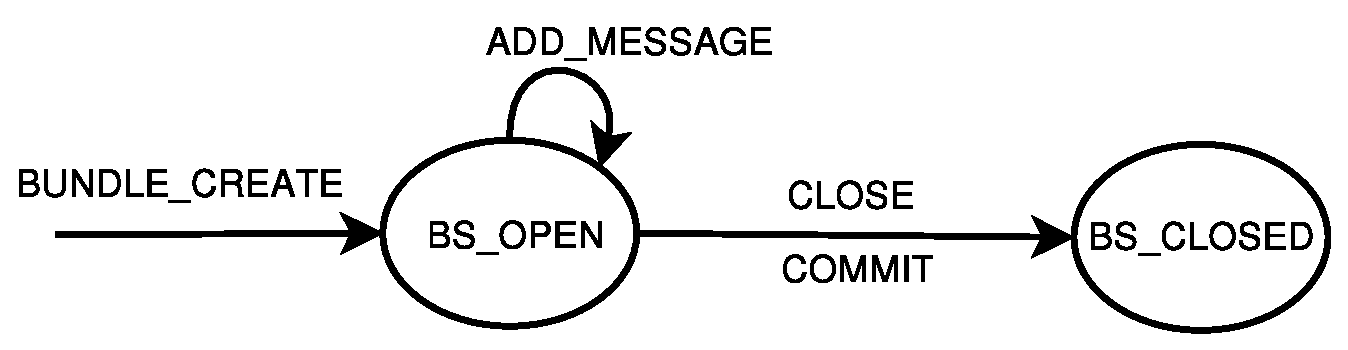
\includegraphics[scale=0.5]{src/img/bundle-state-machine.eps}
\end{center}
\caption{State Transitions of a Bundle}
\label{fig:bundle-state}
\end{figure}

\section{Port Modification Messages}

Each message added to a bundle is checked and the decoded version is cached in a list of messages.
For port-mod messages, the staging area is made of copies of \texttt{struct ofport} representing the ports that
will be modified by each message in a bundle. These structures are linked in a list and attached to the corresponding bundle.
The specification says that when the flag \texttt{OFPBF_ORDERED} is used, the messages should be processed in order.
However, we do this always, the port data structures are modified iteratively by each message in the bundle.

At the commit phase, we apply the changes in the
staging area to the switch and send the needed notifications. From the point of view of the controller, there was only
one operation that did all the changes together. This is possible for port-mod messages because the modified values are mostly
flags so we can easily merge them together with binary operations. These flags are then pushed down to the underlying
network device which controls the configured port.

\section{Flow Modification Messages}

Handling flow-mod messages in a bundle is more difficult because the changes are spread in multiple parts of the switch.
We cannot create the same type of staging area that we used for port-mod messages. Moreover, flow-mod messages can have
different actions, like adding, modifying or removing flows and so they have to be treated differently.

Adding flows is done by using higher priorities instead of the original priority found in the flow-mod message. This
will force the switch to hide the newly added rule from controllers and will also avoid sending notifications about it.
When we are ready to commit, the rules can be made visible again. In the same way, modifying can be done in 2 steps:
adding new hidden flows and removing the old ones. The actual removing is done only at the time of the commit.

To make sure that the data structures that are to be modified by the messages in a bundle won't change or even disappear,
we had to take care of concurrent accesses. For each OpenFlow connection, while there are bundles active, we enqueue the
received OpenFlow messages. Bundle control messages are still allowed to pass through. When no more bundles are associated
with a connection, the processing loop will start to extract messages from the queue, if it's not empty.